\documentclass[11pt]{article}

% Language setting
\usepackage[turkish]{babel}
\usepackage{pythonhighlight}

\usepackage[a4paper,top=2cm,bottom=2cm,left=2cm,right=2cm,marginparwidth=2cm]{geometry}

% Useful packages
\usepackage{amsmath}
\usepackage{graphicx}
\usepackage[colorlinks=true, allcolors=blue]{hyperref}
\usepackage{verbatim}
\usepackage{fancyhdr} % for header and footer
\usepackage{titlesec}
\usepackage{parskip}

\setlength{\parindent}{0pt}

\titleformat{\subsection}[runin]{\bfseries}{\thesubsection}{1em}{}

\pagestyle{fancy} % activate the custom header/footer

% define the header/footer contents
\lhead{\small{23BLM-4014 Yapay Sinir Ağları Ara Sınav Soru ve Cevap Kağıdı}}
\rhead{\small{Dr. Ulya Bayram}}
\lfoot{}
\rfoot{}

% remove header/footer on first page
\fancypagestyle{firstpage}{
  \lhead{}
  \rhead{}
  \lfoot{}
  \rfoot{\thepage}
}
 

\title{Çanakkale Onsekiz Mart Üniversitesi, Mühendislik Fakültesi, Bilgisayar Mühendisliği Akademik Dönem 2022-2023\\
Ders: BLM-4014 Yapay Sinir Ağları/Bahar Dönemi\\ 
ARA SINAV SORU VE CEVAP KAĞIDI\\
Dersi Veren Öğretim Elemanı: Dr. Öğretim Üyesi Ulya Bayram}
\author{%
\begin{minipage}{\textwidth}
\raggedright
Öğrenci Adı Soyadı: Ebu Belk AKYILDIZ\\ % Adınızı soyadınızı ve öğrenci numaranızı noktaların yerine yazın
Öğrenci No: 190401072
\end{minipage}%
}

\date{14 Nisan 2023}

\begin{document}
\maketitle
\vspace{-.5in}
\section*{Açıklamalar:}
\begin{itemize}
    \item Vizeyi çözüp, üzerinde aynı sorular, sizin cevaplar ve sonuçlar olan versiyonunu bu formatta PDF olarak, Teams üzerinden açtığım assignment kısmına yüklemeniz gerekiyor. Bu bahsi geçen PDF'i oluşturmak için LaTeX kullandıysanız, tex dosyasının da yer aldığı Github linkini de ödevin en başına (aşağı url olarak) eklerseniz bonus 5 Puan! (Tavsiye: Overleaf)
    \item Çözümlerde ya da çözümlerin kontrolünü yapmada internetten faydalanmak, ChatGPT gibi servisleri kullanmak serbest. Fakat, herkesin çözümü kendi emeğinden oluşmak zorunda. Çözümlerinizi, cevaplarınızı aşağıda belirttiğim tarih ve saate kadar kimseyle paylaşmayınız. 
    \item Kopyayı önlemek için Github repository'lerinizin hiçbirini \textbf{14 Nisan 2023, saat 15:00'a kadar halka açık (public) yapmayınız!} (Assignment son yükleme saati 13:00 ama internet bağlantısı sorunları olabilir diye en fazla ekstra 2 saat daha vaktiniz var. \textbf{Fakat 13:00 - 15:00 arası yüklemelerden -5 puan!}
    \item Ek puan almak için sağlayacağınız tüm Github repository'lerini \textbf{en geç 15 Nisan 2023 15:00'da halka açık (public) yapmış olun linklerden puan alabilmek için!}
    \item \textbf{14 Nisan 2023, saat 15:00'dan sonra gönderilen vizeler değerlendirilmeye alınmayacak, vize notu olarak 0 (sıfır) verilecektir!} Son anda internet bağlantısı gibi sebeplerden sıfır almayı önlemek için assignment kısmından ara ara çözümlerinizi yükleyebilirsiniz yedekleme için. Verilen son tarih/saatte (14 Nisan 2023, saat 15:00) sistemdeki en son yüklü PDF geçerli olacak.
    \item Çözümlerin ve kodların size ait ve özgün olup olmadığını kontrol eden bir algoritma kullanılacaktır. Kopya çektiği belirlenen vizeler otomatikman 0 (sıfır) alacaktır. Bu nedenle çözümlerinizi ve kodlarınızı yukarıda sağladığım gün ve saatlere kadar kimseyle paylaşmayınız.
    \item Bu vizeden alınabilecek en yüksek not 100'dür. Toplam aldığınız puan 100'ü geçerse, aldığınız not 100'e sabitlenecektir.
    \item LaTeX kullanarak PDF oluşturanlar öz geçmişlerine LaTeX bildiklerini de eklemeyi unutmasınlar :)
    \item Bu vizedeki soruların çözümleri ve tex dosyası için istediğiniz kadar sayıda Github repository'si oluşturabilirsiniz. Sadece yukarıda belirttiğim tarihlerde (14 Nisan 2023 saat 15:00 ile 15 Nisan 2023 saat 15:00 arasında) public yapmayı/halka açmayı ve Github profilinizi de öz geçmişinize eklemeyi unutmayın :)
    \item Bilgisayarınıza hiçbir program kurmadan, Overleaf, Google Colab, Kaggle gibi ortamlar üzerinden bu vizeyi tamamlamanız mümkün. İyi çalışmalar!!
\end{itemize}

(Ekstra 5 puan) \url{OdevinTexDosyasınınGithubLinkiniburayakoyun.com}

\newpage
\section{(Toplam 10 Puan) Hopfield Networks:}

\subsection{(2 Puan)} \textbf{ChatGPT’ye size Hopfield Network’ler ile ilgili detaylı bilgi vermesini isteyin. Sorduğunuz soruyu, ChatGPT'nin çıkartığı cevabı aşağı koyun. Bu cevapta anlamadığınız terimleri de ChatGPT’ye sorup, sorduğunuz soruları ve ChatGPT’nin verdiği cevapları da sırayla aşağı koyun.}

    Hopfield ağları, içinde bulunan düğümler (nöronlar) arasındaki etkileşimlere dayalı bir tür geri beslemeli sinir ağıdır. Bu ağlar, birçok uygulama alanında kullanılır, özellikle hatırlama, desen tanıma ve optimizasyon gibi problemleri çözmek için kullanılır.
    
    Hopfield ağları, bir enerji fonksiyonu kullanarak nöronların durumlarını temsil eder. Bu enerji fonksiyonu, ağın toplam enerjisini temsil eder ve nöronların durumlarına bağlı olarak belirlenir. Ağın enerji fonksiyonu, nöronların girdi ağırlıklarına ve aktivasyon fonksiyonlarına dayanır.
    
    Hopfield ağları, asenkron (tek tek nöronların güncellenmesi) veya senkron (tüm nöronların aynı anda güncellenmesi) olarak güncellenebilir. Güncelleme süreci, enerji fonksiyonunun azaltılması amacıyla iteratif olarak gerçekleştirilir.
    Hopfield ağları, otomatik olarak düşük enerji seviyelerinde sabit durumlara ulaşma eğilimindedir. Bu özellikleri nedeniyle, hafızayı hatırlama ve desen tanıma gibi uygulamalarda kullanılabilirler. Özellikle, eksik veya bozulmuş bir giriş desenine dayalı olarak tam bir desenin hatırlanmasını başarabilirler. Bu özelliği, hatalı veya eksik verilerin düzeltilmesi, desen tamamlama ve desen eşleme gibi uygulamalarda kullanılabilir kılar.
    
    Hopfield ağları, düşük güçlü donanım uygulamaları, paralel işlem ve optimize edilmiş hesaplamalar gibi alanlarda da kullanılabilir. Bununla birlikte, büyük veri kümesi veya karmaşık problemlerle başa çıkmak için sınırlı kapasiteleri nedeniyle sınırlamaları bulunmaktadır.
    
    Sonuç olarak, Hopfield ağları, hafıza ve desen tanıma gibi uygulamalarda kullanılan geri beslemeli sinir ağı modelleridir. Enerji fonksiyonları ve güncelleme süreçleri gibi temel prensipleri ile öne çıkarlar ve sınırlı kapasitelerine rağmen belirli uygulamalarda kullanışlı olabilirler.

\textbf{- Geri beslemeli sinir ağı nedir?}

    Geri beslemeli sinir ağı, sinir ağlarındaki nöronların çıktılarının, ağın girişine geri dönmesine izin veren bir ağ yapısıdır. Yani, ağın çıktısı, ağın girişine geri besleme yapılarak kullanılır ve bu geri besleme, ağın davranışını etkiler.
    
    Geri beslemeli sinir ağları, çıktıların anlamlı bir şekilde geri dönmesine izin vererek, ağın daha önceki durumlarına bağlı olarak gelecekteki çıktıları etkileyebilir. Bu, ağın dinamik ve zamanla değişen süreçleri modelleyebilmesine olanak tanır. Geri beslemeli sinir ağları, zaman serileri, kontrol sistemleri, tahmin ve kestirim problemleri gibi alanlarda kullanılabilir.
    
    Geri beslemeli sinir ağları, birçok farklı mimari ve model içerebilir, örneğin Recurrent Sinir Ağları (RNN), Long Short-Term Memory (LSTM) ve Gated Recurrent Unit (GRU) gibi popüler RNN türleri. Bu tür ağlar, geçmiş zaman adımlarından gelen bilgileri hatırlayabilir ve bu bilgilere dayalı olarak güncel çıktıları hesaplayabilir. Bu, zaman içinde değişen veri akışları veya zaman serileri gibi problemleri çözmek için kullanışlıdır.
    
    Geri beslemeli sinir ağları, bilgi işlemde geri beslemenin kullanıldığı durumlarda etkilidir. Örneğin, bir sistem, çıktıların gelecekteki durumlarını hesaplamak için mevcut çıktıları kullanarak kendini güncelleyebilir veya bir dizi adım boyunca bir sonraki adımın tahminini yapabilir. Bu tür ağlar, girişlerin geçmiş durumlarına bağlı olarak anlamlı sonuçlar elde etmek için geri beslemenin gerektiği problemleri çözmek için kullanılır.
    
    Geri beslemeli sinir ağları, dil işleme, zaman serisi tahmini, duygu analizi, konuşma tanıma ve kontrol sistemleri gibi birçok uygulama alanında kullanılmaktadır. Ancak, geri beslemeli sinir ağları karmaşık yapılara sahip olabilir ve eğitimi zor olabilir. Ayrıca, aşırı uyum (overfitting) ve yakınsama sorunları gibi zorlukları da içerebilir. Bu nedenle, doğru model seçimi, eğitim veri kümesi ve hiper parametre ayarlamaları gibi faktörler dikkate alınmalıdır.

\textbf{- Enerji fonksiyonu nedir?}

    Enerji fonksiyonu, bir sistemdeki durumun enerjisel bir temsilidir. Genellikle istatistiksel fizik, makine öğrenimi, yapay zeka, optimizasyon ve diğer birçok alanda kullanılan bir kavramdır. Enerji fonksiyonu, bir sistemdeki durumun enerji seviyesini veya potansiyelini ifade eder ve sistemin hangi durumların tercih edildiğini belirleyen bir kriterdir.
    
    Enerji fonksiyonu, sistemin durumunu temsil eden değişkenlerin bir fonksiyonu olarak ifade edilir. Bu değişkenler, sistemdeki parçacıkların konumları, hızları, spinleri, elektronik durumları gibi olabilir. Enerji fonksiyonu, bu değişkenlere göre hesaplanan bir skordur ve sistemdeki durumun enerjisel stabilite veya istikrarını yansıtır. Düşük enerji seviyeleri, sistemin daha istikrarlı ve tercih edilen durumlarına karşılık gelirken, yüksek enerji seviyeleri ise daha az tercih edilen veya istikrarsız durumlarına karşılık gelir.
    
    Enerji fonksiyonları, genellikle belirli bir problem veya modelin matematiksel temelini oluşturur. Örneğin, bir Hopfield ağı veya Ising modeli gibi bazı fiziksel veya yapay zeka modellerinde enerji fonksiyonları kullanılır. Enerji fonksiyonları, sistemin davranışını ve dinamiklerini tanımlar ve bu fonksiyonlar üzerinden sistem davranışının analiz edilmesi, optimizasyon ve çeşitli tahminlerin yapılması gibi çeşitli uygulamaları vardır.
    
    Enerji fonksiyonları, çeşitli matematiksel tekniklerle tanımlanabilir ve genellikle deney veya veri kullanılarak belirlenir. Enerji fonksiyonları, genellikle sistemin enerjiyi minimize etmeye veya maksimize etmeye çalıştığı enerji tabanlı modellere temel oluşturur ve bu modeller, birçok alanda kullanılır.



\subsection{(8 Puan)} \textbf{ChatGPT’nin açıklamalarından ne anladığınızı buraya kendi kelimelerinizle özetleyin. Örneğin ``Hopfield Network nedir? Ne işe yarar? Neden bilmemiz gerekir bunu? Gerçek hayatta kullanılıyor mu?'' gibi. Anlamadığınız kısımlar varsa ve ChatGPT’nin açıklamaları yeterli gelmezse internet dahil farklı kaynaklardan araştırıp, bilgilerin doğruluğunu sorgulamakta serbestsiniz. Konuyu doğru anlayıp anlamamanız puana etki edecektir. Kullandığınız kaynakları da belirtin!}

Hopfield Network, yapay sinir ağıdır ve hafıza, hatırlama ve optimizasyon problemlerini çözmek için kullanılır. Gerçek hayatta, karakter tanıma, hatalı veri düzeltme, veri sıkıştırma, robotik, moleküler tasarım, trafik yönetimi ve finansal modelleme gibi alanlarda kullanım potansiyeli bulunan bir yapay sinir ağıdır. Hopfield Network, yapay zeka ve makine öğrenimi alanında çalışanlar için önemlidir çünkü karmaşık problemleri çözmek için etkili bir yaklaşım sunar. Gerçek hayatta Google’ın BERT modeli doğal dil işleme için Hopfield Network yapay sinir ağına benzer bir mekanizma kullanıyor. Hopfield Network için beğendiğim özelliklerinden birisi bozuk veya eksik verilerden orijinal verileri yeniden oluşturabilecek bir yapay sinir ağı olmasıdır. Örneğin, bir resmin parçalarını veya gürültülü bir versiyonunu Hopfield Network yapay sinir ağına verirsek, ağ bize tam ve temiz bir resim döndürebilir.

\section{(Toplam 10 Puan) Boltzman Machine:}

\subsection{(2 Puan)} \textbf{ChatGPT’ye size Boltzman Machine ilgili detaylı bilgi vermesini isteyin. Sorduğunuz soruyu, ChatGPT'nin çıkartığı cevabı aşağı koyun. Bu cevapta anlamadığınız terimleri de ChatGPT’ye sorup, sorduğunuz soruları ve ChatGPT’nin verdiği cevapları da sırayla aşağı koyun.}

Boltzmann Machine, istatistiksel bir makine öğrenimi modelidir ve olasılık tabanlı bir enerji fonksiyonu kullanarak veri kümesindeki gizli yapıları ve istatistiksel dağılımları yakalayabilir. BM, 1980'lerde Geoff Hinton ve Terry Sejnowski tarafından tanıtılmıştır ve sinir ağı tabanlı bir model olarak bilinir.

Boltzmann Machine, iki tip birim içerir: görünür birimler (visible units) ve gizli birimler (hidden units). Görünür birimler, modele dışarıdan verilen girdi verilerini temsil ederken, gizli birimler, verinin öğrenildiği ve modelin karmaşıklığını yakaladığı katmanı temsil eder. Bu birimler arasındaki bağlantılar, enerji fonksiyonu kullanılarak ifade edilir ve ağırlıklar rastgele başlatılır.

Boltzmann Machine, bir veri kümesine dayalı istatistiksel dağılımları yakalamak için iki temel süreç olan öğrenme (learning) ve çıkarım (inference) aşamalarını içerir:

Öğrenme (Learning): BM, veri kümesindeki dağılımları öğrenmek için öğrenme algoritmaları kullanır. Genellikle Markov Zinciri Monte Carlo (MCMC) yöntemleri, Gibbs Örnekleme gibi yöntemler kullanılır. Bu süreçte, ağdaki ağırlıklar güncellenir ve veri kümesine uygun bir enerji fonksiyonu yakalanmaya çalışılır.

Çıkarım (Inference): BM, veri kümesindeki gizli yapıları keşfetmek için çıkarım (inference) işlemini kullanır. çıkarım işlemi, ağdaki birimler arasındaki etkileşimlerin iteratif bir şekilde güncellenmesi ile gerçekleştirilir. Bu süreçte, modele verilen girdiye karşılık gelen olasılık dağılımları elde edilir.

Boltzmann Machine, çeşitli uygulama alanlarında kullanılabilir. Özellikle, özellik çıkarımı, anomali tespiti, tavsiye sistemleri ve rastgele örnek üretimi gibi alanlarda kullanışlıdır. BM, gerçek hayatta kullanımı sınırlı olsa da, temel prensipleri ve olasılık tabanlı enerji fonksiyonu gibi konseptleri, makine öğrenimi ve istatistiksel modeller konusunda daha genel bir anlayış geliştirmek için önemlidir. Ayrıca, BM'nin daha gelişmiş yapay sinir ağı modellerinin temelini oluşturduğu düşünülmektedir.

\textbf{- Inference nedir?}

"Inference" (çıkarım), veri analitiği ve makine öğrenimi alanında, mevcut veri ve modeller kullanılarak yeni veri noktalarının veya sonuçların tahmin edilmesini ifade eder. Başka bir deyişle, mevcut bilgiler ve öğrenilmiş modeller temel alınarak sonuçlara veya sonuçlara varma sürecidir.

Makine öğrenimi ve istatistikte, çıkarım genellikle eğitim verileri üzerinde öğrenilen bir modelin kullanılarak yeni veri noktalarının tahmin edilmesini içerir. Eğitim verileri, modelin parametrelerini belirlemek için kullanılan veri kümesidir ve model, eğitim verilerine dayalı olarak örüntüleri veya ilişkileri yakalamak için ayarlanır. Daha sonra, model, eğitim verilerinden farklı ancak benzer yapıdaki yeni veri noktaları üzerinde tahminlerde bulunabilir.

Çıkarım, bir modelin gerçek dünya verilerine uygulanabilir hale getirilmesini sağlar. Öğrenilmiş model, gerçek verileri kullanarak tahminlerde bulunabilir, sınıflandırma, regresyon, nesne tespiti, doğal dil işleme ve diğer birçok uygulamada kullanılabilir.

Örneğin, bir görüntü sınıflandırma modeli, eğitim verileri üzerinde eğitildikten sonra yeni görüntülerde hangi sınıfa ait olduklarını tahmin etmek için çıkarım yapabilir. Benzer şekilde, bir dil modeli, öğrenildikten sonra yeni metinlerde dil bilgisi hatalarını düzeltmek veya metni anlamak için çıkarım yapabilir.

Çıkarım, makine öğrenimi ve veri analitiğinde önemli bir adımdır, çünkü modellerin gerçek dünya verilerine uygulanabilmesini ve kullanılabilir sonuçlar üretebilmesini sağlar.

\subsection{(8 Puan)} \textbf{ChatGPT’nin açıklamalarından ne anladığınızı buraya kendi kelimelerinizle özetleyin. Örneğin ``Boltzman Machine nedir? Ne işe yarar? Neden bilmemiz gerekir bunu? Gerçek hayatta kullanılıyor mu?'' gibi. Anlamadığınız kısımlar varsa ve ChatGPT’nin açıklamaları yeterli gelmezse internet dahil farklı kaynaklardan araştırıp, bilgilerin doğruluğunu sorgulamakta serbestsiniz. Konuyu doğru anlayıp anlamamanız puana etki edecektir. Kullandığınız kaynakları da belirtin!}

Boltzmann Machine, olasılıklı bir enerji tabanlı modeldir. İstatistiksel makine öğrenimi alanında kullanılan bir tür yapay sinir ağıdır. Boltzmann Machine, gizli ve görünür katmanlardan oluşan bir yapay sinir ağıdır ve genellikle olasılıklı örüntülerin modellenmesi, veri analitiği, doğal dil işleme ve diğer birçok alanda kullanılır. Boltzmann Makineleri, rastgele değişkenlerle enerji fonksiyonunu minimize eden bir modeldir. Boltzmann Makineleri, model parametrelerinin öğrenilmesi ve olasılıksal çıkarımlar yapma yeteneği ile önemli bir yapay sinir ağıdır.

\section{(Toplam 10 Puan) Markov Assumption ve Markov Chain:}

\subsection{(2 Puan)} \textbf{ChatGPT’ye size Markov assumption ve Markov Chain ilgili detaylı bilgi vermesini isteyin. Sorduğunuz soruyu, ChatGPT'nin çıkartığı cevabı aşağı koyun. Bu cevapta anlamadığınız terimleri de ChatGPT’ye sorup, sorduğunuz soruları ve ChatGPT’nin verdiği cevapları da sırayla aşağı koyun.}

Markov Assumption ve Markov Chain, olasılık teorisi ve istatistiklerde önemli kavramlardır.

Markov Assumption: Markov Assumption, bir sürecin gelecekteki durumunun yalnızca şu anki durumuna bağlı olduğunu ve geçmiş durumların süreç için önemsiz olduğunu varsayar. Matematiksel olarak, bir sürecin Markov olması için, "geçmiş bağımsızlığı" olarak da adlandırılan Markov Assumption sağlanması gerekmektedir. Yani, bir süreçte, bir sonraki durumun olasılığı, sadece mevcut durumunun bilgisine bağlıdır ve geçmiş durumlar sürece etki etmez.

Markov Chain: Markov Chain, Markov Assumption tabi olan bir olasılık sürecidir. Bir Markov Chain, belirli bir durum kümesi ve bu durumlar arasındaki geçiş olasılıklarını içerir. Herhangi bir durumun gelecekteki durumu, sadece o anki durum ve geçiş olasılıklarıyla belirlenir. Matematiksel olarak, Markov Chain, "gelecek, geçmişe bağlı değildir" şeklinde ifade edilebilecek bir olasılık süreçidir.

Markov Chain, zamanla değişen durumlarını modellemek için kullanılan matematiksel bir araçtır ve bir dizi durum arasında geçiş olasılıklarını kullanarak gelecekteki durumların olasılık dağılımlarını tahmin etmek için kullanılabilir. Markov Chain, birçok uygulamada kullanılır, özellikle rastgele süreçleri modellemek, zaman serilerini analiz etmek, sıradan durumlu diferansiyel denklemleri çözmek ve karar verme problemlerini çözmek gibi alanlarda yaygın olarak kullanılır.

Markov Chain, doğal dil işleme, finansal piyasalar, biyoinformatik, epidemiyoloji, sosyal ağ analitiği gibi birçok alanda uygulama bulmuştur. Örneğin, hava durumu tahmininde, hisse senedi fiyatlarının modellemesinde, hastalık yayılımının tahmininde, kullanıcı davranışlarının analizinde ve daha birçok alanda Markov Chain başarılı bir şekilde kullanılmaktadır.


\subsection{(8 Puan)} \textbf{ChatGPT’nin açıklamalarından ne anladığınızı buraya kendi kelimelerinizle özetleyin. Örneğin ``Markov assumption ve Markov Chain nedir? Ne işe yarar? Neden bilmemiz gerekir bunu? Gerçek hayatta kullanılıyor mu?'' gibi. Anlamadığınız kısımlar varsa ve ChatGPT’nin açıklamaları yeterli gelmezse internet dahil farklı kaynaklardan araştırıp, bilgilerin doğruluğunu sorgulamakta serbestsiniz. Konuyu doğru anlayıp anlamamanız puana etki edecektir. Kullandığınız kaynakları da belirtin!}

Markov Assumption, bir sürecin gelecekteki durumunu tahmin ederken sadece anlık durumunun dikkate alınması anlamına gelir. Yani geçmiş veya gelecek durumlarla ilgilenmez, sadece mevcut duruma bakar. Markov Chain ise, bir sürecin gelecekteki durumunu tahmin etmek için kullanılan bir modeldir.

Markov Chain, pek çok uygulama alanında kullanılır. Özellikle zaman serileri analizi, doğal dil işleme, finans, trafik akışı modellemesi, hava durumu tahminleri gibi alanlarda kullanılır. Ayrıca, rastgele süreçleri modellemede, sistemlerin dinamik davranışını anlamada ve belirsizlik içeren problemleri çözmede de kullanılabilir. Markov Chain anlaşılması ve kullanılması, bu alanlarda çalışan veri bilimciler, istatistikçiler, mühendisler ve araştırmacılar için önemlidir.



\section{(Toplam 20 Puan) Feed Forward:}
 
\begin{itemize}
    \item Forward propagation için, input olarak şu X matrisini verin (tensöre çevirmeyi unutmayın):\\
    $X = \begin{bmatrix}
        1 & 2 & 3\\
        4 & 5 & 6
        \end{bmatrix}$
    Satırlar veriler (sample'lar), kolonlar öznitelikler (feature'lar).
    \item Bir adet hidden layer olsun ve içinde tanh aktivasyon fonksiyonu olsun
    \item Hidden layer'da 50 nöron olsun
    \item Bir adet output layer olsun, tek nöronu olsun ve içinde sigmoid aktivasyon fonksiyonu olsun
\end{itemize}

Tanh fonksiyonu:\\
$f(x) = \frac{exp(x) - exp(-x)}{exp(x) + exp(-x)}$
\vspace{.2in}

Sigmoid fonksiyonu:\\
$f(x) = \frac{1}{1 + exp(-x)}$

\vspace{.2in}
 \textbf{Pytorch kütüphanesi ile, ama kütüphanenin hazır aktivasyon fonksiyonlarını kullanmadan, formülünü verdiğim iki aktivasyon fonksiyonunun kodunu ikinci haftada yaptığımız gibi kendiniz yazarak bu yapay sinir ağını oluşturun ve aşağıdaki üç soruya cevap verin.}
 
\subsection{(10 Puan)} \textbf{Yukarıdaki yapay sinir ağını çalıştırmadan önce pytorch için Seed değerini 1 olarak set edin, kodu aşağıdaki kod bloğuna ve altına da sonucu yapıştırın:}

% Latex'de kod koyabilirsiniz python formatında. Aşağıdaki örnekleri silip içine kendi kodunuzu koyun
\begin{python}
import torch
import torch.nn as nn

# Seed " 1 " olarak tanimlanmasi
torch.manual_seed(1)

# X matrisini PyTorch Tensor formatina donusturulmesi
X = torch.tensor([[1, 2, 3 ],[4, 5, 6]], dtype = torch.float32)

# Aktivasyon fonksiyonlarinin tanimlanmasi
def tanh(x):
  return(torch.exp(x) - torch.exp(-x)) / (torch.exp(x) + torch.exp(-x))

def sigmoid(x):
  return 1 / ( 1 + torch . exp ( - x ) )

# Sinir agi modelinin tanimlanmasi
class MyModel ( nn . Module ) :
  def __init__ (self):
    super (MyModel, self).__init__()
    self.hidden_layer = nn.Linear (3, 50) # 3 girdi ozelliginden 50 gizli norona gecis yapacak
    self.output_layer = nn.Linear (50, 1) # 50 gizli norandan 1 cikti norona gecis yapacak
  def forward (self, x):
    hidden = tanh(self.hidden_layer(x)) # Gizli katmani uygula
    output = sigmoid(self.output_layer(hidden)) # Cikti katmanini uygula
    return output
    
# Modelin olusturulmasi
model = MyModel()
# Forward Propagation ’u uygulanmasi
output = model(X)
print(output)
\end{python}

tensor([[0.4892],
        [0.5566]])

\subsection{(5 Puan)} \textbf{Yukarıdaki yapay sinir ağını çalıştırmadan önce Seed değerini öğrenci numaranız olarak değiştirip, kodu aşağıdaki kod bloğuna ve altına da sonucu yapıştırın:}

\begin{python}
import torch
import torch.nn as nn

# Seed " 190401072 " olarak tanimlanmasi
torch.manual_seed(190401072)

# X matrisini PyTorch Tensor formatina donusturulmesi
X = torch.tensor([[1, 2, 3 ],[4, 5, 6]], dtype = torch.float32)

# Aktivasyon fonksiyonlarinin tanimlanmasi
def tanh(x):
  return(torch.exp(x) - torch.exp(-x)) / (torch.exp(x) + torch.exp(-x))

def sigmoid(x):
  return 1 / ( 1 + torch . exp ( - x ) )

# Sinir agi modelinin tanimlanmasi
class MyModel ( nn . Module ) :
  def __init__ (self):
    super (MyModel, self).__init__()
    self.hidden_layer = nn.Linear (3, 50) # 3 girdi ozelliginden 50 gizli norona gecis yapacak
    self.output_layer = nn.Linear (50, 1) # 50 gizli norandan 1 cikti norona gecis yapacak
  def forward (self, x):
    hidden = tanh(self.hidden_layer(x)) # Gizli katmani uygula
    output = sigmoid(self.output_layer(hidden)) # Cikti katmanini uygula
    return output
    
# Modelin olusturulmasi
model = MyModel()
# Forward Propagation’u uygulanmasi
output = model(X)
print(output)
\end{python}

tensor([[0.5820],
        [0.6434]])

\subsection{(5 Puan)} \textbf{Kodlarınızın ve sonuçlarınızın olduğu jupyter notebook'un Github repository'sindeki linkini aşağıdaki url kısmının içine yapıştırın. İlk sayfada belirttiğim gün ve saate kadar halka açık (public) olmasın:}
% size ait Github olmak zorunda, bu vize için ayrı bir github repository'si açıp notebook'u onun içine koyun. Kendine ait olmayıp da arkadaşının notebook'unun linkini paylaşanlar 0 alacak.

\url{https://github.com/ebubelk/MyModel_FFP.git}

\section{(Toplam 40 Puan) Multilayer Perceptron (MLP):} 
\textbf{Bu bölümdeki sorularda benim vize ile beraber paylaştığım Prensesi İyileştir (Cure The Princess) Veri Seti parçaları kullanılacak. Hikaye şöyle (soruyu çözmek için hikaye kısmını okumak zorunda değilsiniz):} 

``Bir zamanlar, çok uzaklarda bir ülkede, ağır bir hastalığa yakalanmış bir prenses yaşarmış. Ülkenin kralı ve kraliçesi onu iyileştirmek için ellerinden gelen her şeyi yapmışlar, ancak denedikleri hiçbir çare işe yaramamış.

Yerel bir grup köylü, herhangi bir hastalığı iyileştirmek için gücü olduğu söylenen bir dizi sihirli malzemeden bahsederek kral ve kraliçeye yaklaşmış. Ancak, köylüler kral ile kraliçeyi, bu malzemelerin etkilerinin patlayıcı olabileceği ve son zamanlarda yaşanan kuraklıklar nedeniyle bu malzemelerden sadece birkaçının herhangi bir zamanda bulunabileceği konusunda uyarmışlar. Ayrıca, sadece deneyimli bir simyacı bu özelliklere sahip patlayıcı ve az bulunan malzemelerin belirli bir kombinasyonunun prensesi iyileştireceğini belirleyebilecekmiş.

Kral ve kraliçe kızlarını kurtarmak için umutsuzlar, bu yüzden ülkedeki en iyi simyacıyı bulmak için yola çıkmışlar. Dağları tepeleri aşmışlar ve nihayet "Yapay Sinir Ağları Uzmanı" olarak bilinen yeni bir sihirli sanatın ustası olarak ün yapmış bir simyacı bulmuşlar.

Simyacı önce köylülerin iddialarını ve her bir malzemenin alınan miktarlarını, ayrıca iyileşmeye yol açıp açmadığını incelemiş. Simyacı biliyormuş ki bu prensesi iyileştirmek için tek bir şansı varmış ve bunu doğru yapmak zorundaymış. (Original source: \url{https://www.kaggle.com/datasets/unmoved/cure-the-princess})

(Buradan itibaren ChatGPT ve Dr. Ulya Bayram'a ait hikayenin devamı)

Simyacı, büyülü bileşenlerin farklı kombinasyonlarını analiz etmek ve denemek için günler harcamış. Sonunda birkaç denemenin ardından prensesi iyileştirecek çeşitli karışım kombinasyonları bulmuş ve bunları bir veri setinde toplamış. Daha sonra bu veri setini eğitim, validasyon ve test setleri olarak üç parçaya ayırmış ve bunun üzerinde bir yapay sinir ağı eğiterek kendi yöntemi ile prensesi iyileştirme ihtimalini hesaplamış ve ikna olunca kral ve kraliçeye haber vermiş. Heyecanlı ve umutlu olan kral ve kraliçe, simyacının prensese hazırladığı ilacı vermesine izin vermiş ve ilaç işe yaramış ve prenses hastalığından kurtulmuş.

Kral ve kraliçe, kızlarının hayatını kurtardığı için simyacıya krallıkta kalması ve çalışmalarına devam etmesi için büyük bir araştırma bütçesi ve çok sayıda GPU'su olan bir server vermiş. İyileşen prenses de kendisini iyileştiren yöntemleri öğrenmeye merak salıp, krallıktaki üniversitenin bilgisayar mühendisliği bölümüne girmiş ve mezun olur olmaz da simyacının yanında, onun araştırma grubunda çalışmaya başlamış. Uzun yıllar birlikte krallıktaki insanlara, hayvanlara ve doğaya faydalı olacak yazılımlar geliştirmişler, ve simyacı emekli olduğunda prenses hem araştırma grubunun hem de krallığın lideri olarak hayatına devam etmiş.

Prenses, kendisini iyileştiren veri setini de, gelecekte onların izinden gidecek bilgisayar mühendisi prensler ve prensesler başkalarına faydalı olabilecek yapay sinir ağları oluşturmayı öğrensinler diye halka açmış ve sınavlarda kullanılmasını salık vermiş.''

\textbf{İki hidden layer'lı bir Multilayer Perceptron (MLP) oluşturun beşinci ve altıncı haftalarda yaptığımız gibi. Hazır aktivasyon fonksiyonlarını kullanmak serbest. İlk hidden layer'da 100, ikinci hidden layer'da 50 nöron olsun. Hidden layer'larda ReLU, output layer'da sigmoid aktivasyonu olsun.}

\textbf{Output layer'da kaç nöron olacağını veri setinden bakıp bulacaksınız. Elbette bu veriye uygun Cross Entropy loss yöntemini uygulayacaksınız. Optimizasyon için Stochastic Gradient Descent yeterli. Epoch sayınızı ve learning rate'i validasyon seti üzerinde denemeler yaparak (loss'lara overfit var mı diye bakarak) kendiniz belirleyeceksiniz. Batch size'ı 16 seçebilirsiniz.}

\subsection{(10 Puan)} \textbf{Bu MLP'nin pytorch ile yazılmış class'ının kodunu aşağı kod bloğuna yapıştırın:}

\begin{python}
class MLP(nn.Module):
    def __init__(self):
        super(MLP, self).__init__()
        self.hidden_layer_first = nn.Linear(13, 100)
        self.hidden_layer_second = nn.Linear(100, 50)
        self.output_layer = nn.Linear(50, 1)
        self.relu = nn.ReLU() # ReLU aktivasyonu
        self.sigmoid = nn.Sigmoid() # sigmoid aktivasyonu
        self.dropout_first = nn.Dropout(0.4)
        self.dropout_second = nn.Dropout(0.3)

    def forward(self, x):
        hidden_first = self.relu(self.dropout_first(self.hidden_layer_first(x)))
        hidden_second = self.relu(self.dropout_second(self.hidden_layer_second(hidden_first)))
        output = self.sigmoid(self.output_layer(hidden_second))
        return output
\end{python}
 _\\
\subsection{(10 Puan)} \textbf{SEED=öğrenci numaranız set ettikten sonra altıncı haftada yazdığımız gibi training batch'lerinden eğitim loss'ları, validation batch'lerinden validasyon loss değerlerini hesaplayan kodu aşağıdaki kod bloğuna yapıştırın ve çıkan figürü de alta ekleyin.}

\begin{python}
start = time.time()
# Egitim parametreleri
learning_rate = 0.001
num_epochs = 1000
patience = 10

# Model, loss fonksiyonu ve optimizer olusturma
model = MLP()
model = model.to(device)
criterion = nn.BCELoss()
optimizer = optim.SGD(model.parameters(), lr=learning_rate)

# Egitim dongusu
list_train_loss = []
list_val_loss = []
best_val_loss = None
patience_counter = 0

for epoch in range(num_epochs):
    train_loss = 0.0
    model.train() # train modunda modeli ayarla
    for inputs, labels in trainloader:
        inputs, labels = inputs.to(device), labels.to(device)
        optimizer.zero_grad()
        outputs = model(inputs)
        loss = criterion(outputs, labels)
        loss.backward()
        optimizer.step()
        train_loss += loss.item()
    
    train_loss /= len(trainloader)
    
    # Dogrulama seti uzerinde modelin performansini degerlendirme
    val_loss = 0.0
    model.eval() # eval modunda modeli ayarla
    with torch.no_grad():
        for inputs, labels in valloader:
            inputs, labels = inputs.to(device), labels.to(device)
            outputs = model(inputs)
            loss = criterion(outputs, labels)
            val_loss += loss.item()
    
    val_loss /= len(valloader)
    
    print("Epoch", epoch, "Training loss", train_loss, "Validation Loss :", val_loss)
    
    list_train_loss.append(train_loss)
    list_val_loss.append(val_loss)
    
    val_score = val_loss
    if best_val_loss is None:
        best_val_loss = val_score
        torch.save(model.state_dict(), "checkpoint.pt")
    elif best_val_loss < val_score:
        patience_counter += 1
        print("Earlystopping Patience Counter:", patience_counter)
        if patience_counter == patience:
            print("Early stopping triggered.")
            break
    else:
        best_val_loss = val_score  # en iyi loss'u guncelle
        patience_counter = 0  # patience counter'i sifirla
torch.save(model.state_dict(), "last.pt")

sns.set_style("darkgrid")
plt.plot(list_train_loss, label="Train Loss")
plt.plot(list_val_loss, label="Validation Loss")
plt.xlabel("Epoch")
plt.ylabel("Loss")
plt.legend()
plt.show()
end = time.time()
print("Run time:", end - start)
\end{python}

% Figure aşağıda comment içindeki kısımdaki gibi eklenir.

\begin{figure}[ht!]
    \centering
    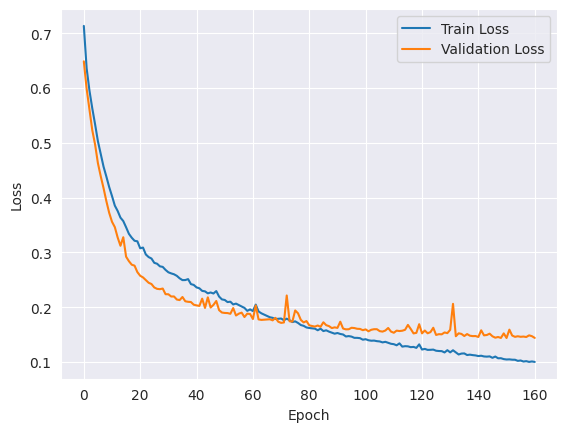
\includegraphics[width=0.7\textwidth]{figure/mlpfigure.png}
    \caption{5.2 sorusu için çıktı}
    \label{fig:mlpfigure}
\end{figure}


\subsection{(10 Puan)} \textbf{SEED=öğrenci numaranız set ettikten sonra altıncı haftada ödev olarak verdiğim gibi earlystopping'deki en iyi modeli kullanarak, Prensesi İyileştir test setinden accuracy, F1, precision ve recall değerlerini hesaplayan kodu yazın ve sonucu da aşağı yapıştırın. \%80'den fazla başarı bekliyorum test setinden. Daha düşükse başarı oranınız, nerede hata yaptığınızı bulmaya çalışın. \%90'dan fazla başarı almak mümkün (ben denedim).}

\begin{python}
device = "cpu"
model.to(device)
model.load_state_dict(torch.load("last.pt"))
model.eval()
test_loss = 0.0
outputs_list = []
with torch.no_grad():
    for inputs, labels in testloader:
        inputs, labels = inputs.to(device), labels.to(device)
        outputs = model(inputs)
        loss = criterion(outputs, labels)
        test_loss += loss.item()
        outputs = (outputs >= 0.5).float()
        outputs_list.append(outputs)
test_loss /= len(testloader)
outputs_list = torch.cat(outputs_list, dim=0).numpy()
test_acc = accuracy_score(test_value, outputs_list)
test_f1 = f1_score(test_value, outputs_list, average='weighted')
test_precision = precision_score(test_value, outputs_list)
test_recall = recall_score(test_value, outputs_list)

print("Test Loss:", test_loss)
print("Test Accuracy:", test_acc)
print("Test F1 Score:", test_f1)
print("Test Precision Score:", test_precision)
print("Test Recall Score:", test_recall)
\end{python}
Test Loss: 0.1433588265992549\\
Test Accuracy: 0.9494818652849741\\
Test F1 Score: 0.9494719465200716\\
Test Precision Score: 0.9653333333333334\\
Test Recall Score: 0.9329896907216495
\subsection{(5 Puan)} \textbf{Tüm kodların CPU'da çalışması ne kadar sürüyor hesaplayın. Sonra to device yöntemini kullanarak modeli ve verileri GPU'ya atıp kodu bir de böyle çalıştırın ve ne kadar sürdüğünü hesaplayın. Süreleri aşağıdaki tabloya koyun. GPU için Google Colab ya da Kaggle'ı kullanabilirsiniz, iki ortam da her hafta saatlerce GPU hakkı veriyor.}

\begin{table}[ht!]
    \centering
    \caption{Farklı ortamların çalışma süreleri}
    \begin{tabular}{c|c}
        Ortam & Süre (saniye) \\\hline
        CPU & 516.75  \\
        GPU & 550.46\\
    \end{tabular}
    \label{tab:my_table}
\end{table}

\subsection{(3 Puan)} 
\textbf{Modelin eğitim setine overfit etmesi için elinizden geldiği kadar kodu gereken şekilde değiştirin, validasyon loss'unun açıkça yükselmeye başladığı, training ve validation loss'ları içeren figürü aşağı koyun ve overfit için yaptığınız değişiklikleri aşağı yazın. Overfit, tam bir çanak gibi olmalı ve yükselmeli. Ona göre parametrelerle oynayın.}
\begin{figure}[ht!]
    \centering
    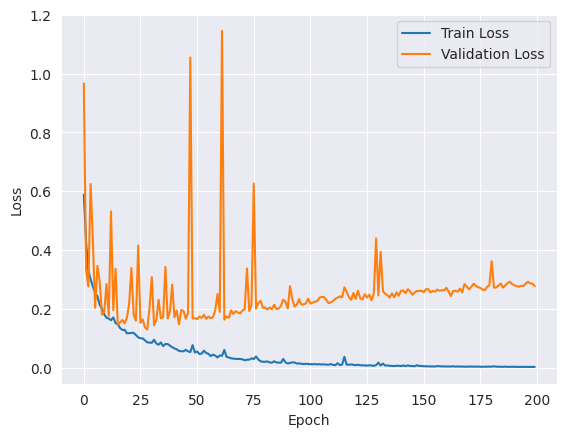
\includegraphics[width=0.7\textwidth]{figure/overfitfigure.png}
    \caption{Overfit çıktı}
    \label{fig:mlpfigure}
\end{figure}

Overfit bir çıktı almak için "learnin rate" değerini arttırdım ve normalde öğrenmesi gereken değerleri aştı. Sabit 200 "epoch" değeri kullandım. "Early stopping" kapattım böylece 200 "epoch" boyunca eğitim yapmış oldu.
\\
\\
\\
\\
\\
\\
\\
\\
\\
\\
\\
\\
\\
\\
\\
% Figür aşağı
\subsection{(2 Puan)} \textbf{Beşinci soruya ait tüm kodların ve cevapların olduğu jupyter notebook'un Github linkini aşağıdaki url'e koyun.}

\url{https://github.com/ebubelk/Cure_The_Princess_MLP.git}\\
Perma Link:\\
\url{https://github.com/ebubelk/Cure_The_Princess_MLP/blob/2a2146802f37b9737c03336c0590bc27f87d4d94/Cure_The_Princess_MLP_Non_Reg.ipynb}

\section{(Toplam 10 Puan)} \textbf{Bir önceki sorudaki Prensesi İyileştir problemindeki yapay sinir ağınıza seçtiğiniz herhangi iki farklı regülarizasyon yöntemi ekleyin ve aşağıdaki soruları cevaplayın.} 

\subsection{(2 puan)} \textbf{Kodlarda regülarizasyon eklediğiniz kısımları aşağı koyun:} 

\textbf{- "Dropout" eklendi:}
\begin{python}
class MLP(nn.Module):
    def __init__(self):
        set_seed(seed=SEED)
        super(MLP, self).__init__()
        self.hidden_layer_first = nn.Linear(13, 100)
        self.hidden_layer_second = nn.Linear(100, 50)
        self.output_layer = nn.Linear(50, 1)
        self.relu = nn.ReLU() # ReLU aktivasyonu
        self.sigmoid = nn.Sigmoid() # sigmoid aktivasyonu
        self.dropout_first = nn.Dropout(0.3)
        self.dropout_second = nn.Dropout(0.2)
        
    def forward(self, x):
        #Add Dropout
        x = self.dropout_first(self.relu(self.hidden_layer_first(x)))
        x = self.dropout_second(self.relu(self.hidden_layer_second(x)))
        x = self.sigmoid(self.output_layer(x))
        return x
\end{python}

\textbf{- L2 regülarizasyon eklendi:}
\begin{python}
# Egitim parametreleri
learning_rate = 0.001
num_epochs = 1000
patience = 10
weight_decay = 0.001 #Add L2 Reg weight_decay

# Model, loss fonksiyonu ve optimizer olusturma
model = MLP()
model = model.to(device)
criterion = nn.BCELoss()
optimizer = optim.SGD(model.parameters(), lr=learning_rate, weight_decay = weight_decay)
\end{python}

\subsection{(2 puan)} \textbf{Test setinden yeni accuracy, F1, precision ve recall değerlerini hesaplayıp aşağı koyun:}

Test Loss: 0.1680730119043467\\
Test Accuracy: 0.9352331606217616\\
Test F1 Score: 0.9351600623159575\\
Test Precision Score: 0.9694444444444444\\
Test Recall Score: 0.8994845360824743
\subsection{(5 puan)} \textbf{Regülarizasyon yöntemi seçimlerinizin sebeplerini ve sonuçlara etkisini yorumlayın:}

"Dropout" ve L2 regülarizasyon ekledim. "Droput" yapay sinir ağı eğitilirken eğitim verilerini ezberlemesini önlüyor. Eğitim için modele gönderilen her veride belirtilen değerlerce nöron açık kalıyor ve o nöronların weight ve bias değerleri güncelleniyor.

L2 regülarizasyon overfiting azaltmak için kullandım. L2 regülarizasyon sayesinde modelin ağırlıkları büyük değerlere ulaşamaz ve overfiting riski azalır.

Bu yöntemler ile birlikte accuary değerlerinde azalmalar gördüm.

\subsection{(1 puan)} \textbf{Sonucun github linkini  aşağıya koyun:}

\url{https://github.com/ebubelk/Cure_The_Princess_MLP.git}\\
Perma Link:\\
\url{https://github.com/ebubelk/Cure_The_Princess_MLP/blob/2a2146802f37b9737c03336c0590bc27f87d4d94/Cure_The_Princess_MLP.ipynb}

\end{document}
